\documentclass{acmsiggraph}
\usepackage{mathptmx}
\usepackage{graphicx}
\usepackage{epsfig}
\usepackage{amsmath,amscd,amssymb}
\usepackage{hyperref}

\newtheorem{theorem}{Theorem}[section]
\newtheorem{proposition}[theorem]{Proposition}
\newtheorem{definition}[theorem]{Definition}
\newtheorem{lemma}[theorem]{Lemma}
\newtheorem{corollary}[theorem]{Corollary}
\newtheorem{remark}[theorem]{Remark}

\usepackage{parskip}
\usepackage{longtable}

\onlineid{papers\_0142}

\acmformat{cameraready}

\title{CS 453/553 Term Project: Visualizing the Loss Landscape of Neural Nets}

\author{Charles Ison\thanks{\small\texttt{e-mail: \{isonc|morgamat\}@eecs.oregonstate.edu}}\\ Oregon State University
\and Matthew Morgan$^{\ast}$ \\
Oregon State University}

\keywords{loss landscape, scalar field topology, neural networks, convolutional neural networks, backpropagation, gradient descent}

\begin{document}

\teaser{
	%\centerline{\epsfig{file=images/teaser.eps,angle=0,width=\textwidth}}
	$\begin{array}{@{\hspace{-0.00in}}c@{\hspace{0.10in}}c@{\hspace{0.10in}}c@{\hspace{0.05in}}c}
		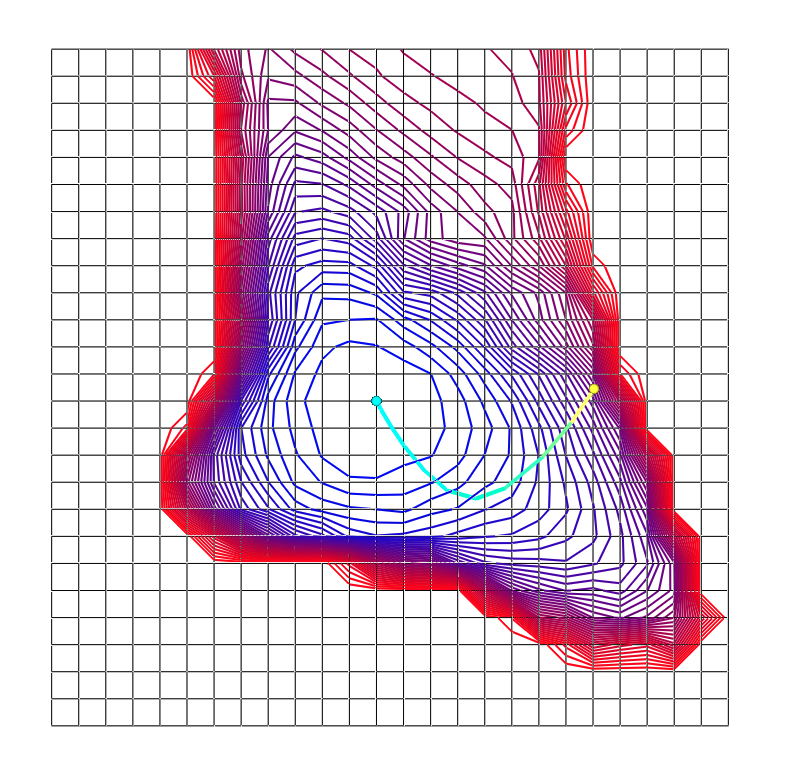
\includegraphics[width=2.2in]{Images/ResNet-PCA-2d-contours.png}
		&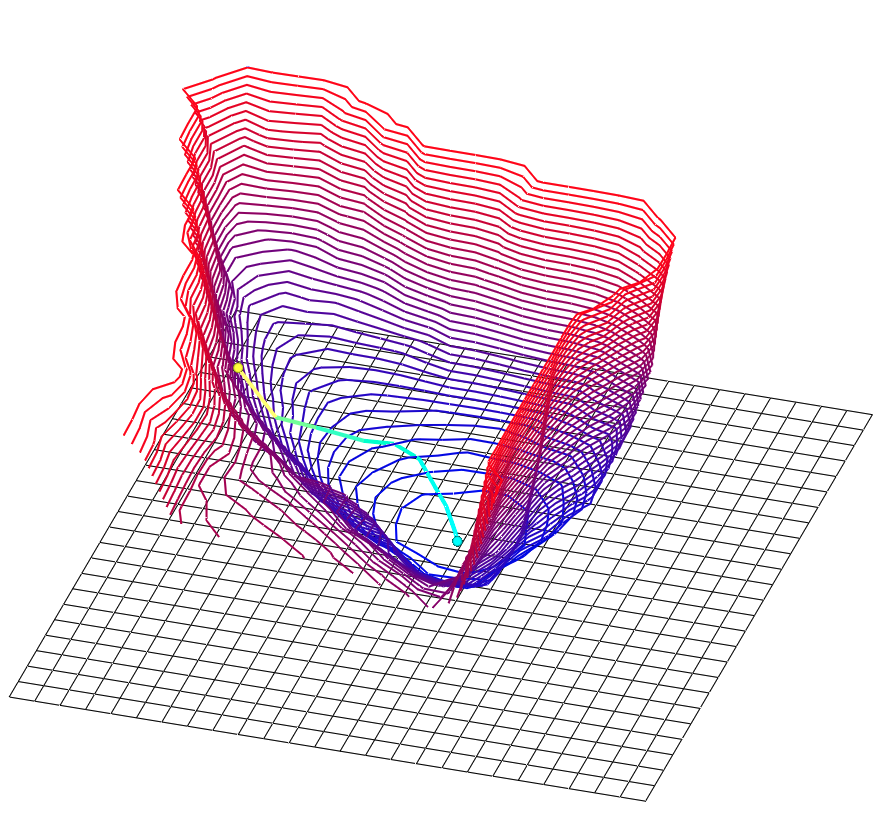
\includegraphics[width=2.2in]{Images/ResNet-PCA-3d-contours.png}
        &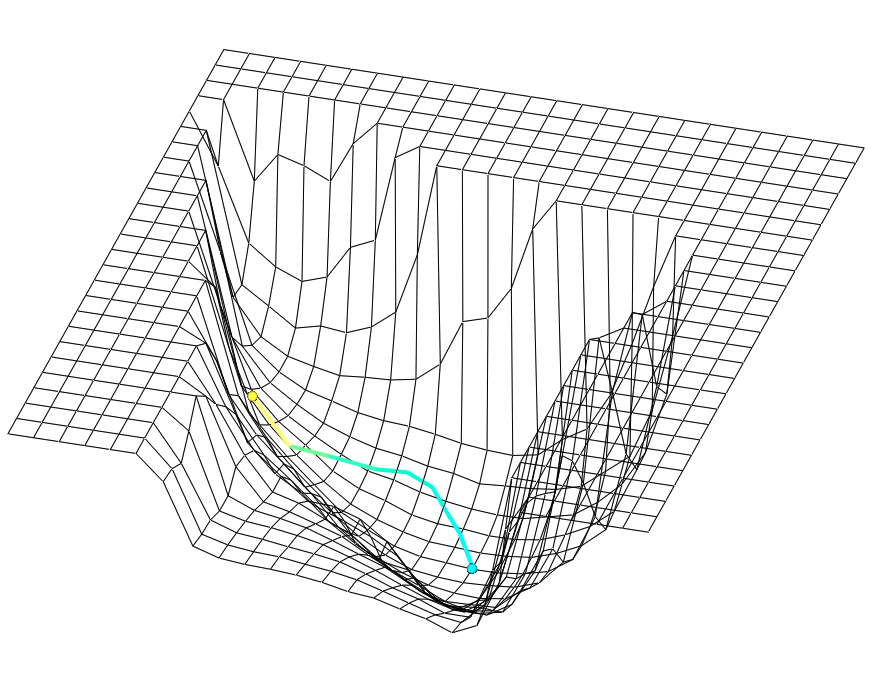
\includegraphics[width=2.2in]{Images/ResNet-PCA-3d-mesh.png}
			\\
			(a)  &  (b) & (c)
		\end{array}$
	\caption{Loss landscapes of the ResNet-50 model from PCA dimensionality reduction, with the gradient decent path. The landscape is visualized in (a) 2D with contours, (b) 3D with contours and mesh base, and (c) 3D with only mesh } \label{fig:teaser} }

\maketitle

\begin{abstract}

	\copyrightspace
    The training of artificial neural networks is a process highly sensitive to architecture choices and hyperparameter tuning. Often these decisions are made by practitioners because it allows them to achieve the best loss for a certain set of parameters and architecture, without a broader understanding of where they are operating within the model's loss landscape. By visualizing both the model's loss landscape and path during gradient descent towards some local minimum, we can gain intuitions about how tuning and architectural decisions impact the model's ability to converge. In this paper, we implement two separate methods proposed by \cite{NEURIPS2018_a41b3bb3}. For each method, we perform dimensionality reduction on a model's weights during backpropagation, then iteratively manipulate the weights using these techniques to generate scalar fields or loss landscapes. Finally, we evaluate our results on two popular neural network models: ResNet-50 and VGG-11.
	
\end{abstract}

%% The ``\keywordlist'' command prints out the keywords.
\keywordlist.

\section{Introduction}
\label{sec:intro}

In the last decade, the use of artificial neural networks for machine learning tasks has proliferated due to rapid gains in available computing power for practitioners. Recent improvements have shown artificial neural networks become the benchmark for many tasks such as image classification and natural language processing \cite{ABIODUN2018e00938}. This success has led to substantial interest in methods that can be used to tune and optimize artificial neural networks. 

One mechanism for cutting through this noise is using loss landscapes to visualize and reason about how hyperparameter tuning and the use of different architectures impact the model's ability to converge. In the paper, "Visualizing the Loss Landscape of Neural Nets" (\url{https://arxiv.org/pdf/1712.09913.pdf}) Li et al. reduce the dimensionality of neural networks weights during different training epochs and then iteratively manipulated the reduced weights to generate intuitive loss landscapes. In this paper, we build off of their work by constructing and training two popular convolutional neural networks (CNNs): ResNet-50 and VGG-11, and adding our own visualizations of the loss landscapes in OpenGL.

We constructed our CNNs in Python using the PyTorch library, then trained and tested our models on the CIFAR-10 dataset (\url{https://www.cs.toronto.edu/~kriz/cifar.html}). The CIFAR-10 dataset is a collection of 6000 color images that are 32x32 pixels and contain 10 separate classes (see Figure 2 for examples). The models were then trained using a batch size of 10 for 10 training epochs and evaluated using cross entropy as the loss function (\url{https://pytorch.org/docs/stable/generated/torch.nn.CrossEntropyLoss.html}).

\begin{figure}[t]
	\begin{center}
		$\begin{array}{@{\hspace{-0.00in}}c@{\hspace{0.05in}}c}
			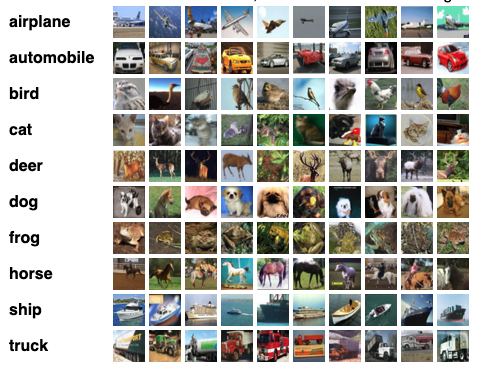
\includegraphics[width=3.5in]{Images/ciphar-10-dataset-example.png}
			\end{array}$
	\end{center}
	\caption{Series of example images from the CIPHAR-10 dataset } \label{fig:coparison_of_landscapes}
\end{figure}

\section{Previous Work}
\label{sec:previous_work}

Although there have been many studies on optimizing artificial neural networks in order to improve training time and model performance, less work has been conducted on visualizing the losses to gain intuition about how these decisions impact the loss field's convexity. One of the earlier works in the space was published in 1997 by ~\cite{hochreiter1997flat}. The authors defined the “flatness” of a loss landscape as the size of the connected region around the minimum where the training loss remains low. Visualizations were then built to show "flatness" to better understand the areas where artificial neural nets minimize loss. In the time since then, technology rapidly advanced, and along with it the complexity of neural networks. The paper we are implementing, "Visualizing the Loss Landscape of Neural Nets", is one of the first to visualize the loss landscapes of modern architectures using both normalized random direction iteration and PCA as dimensionality reduction techniques. Since the paper was released in 2018, numerous other works have cited it. However, many of the citations are not from works attempting to advance the visualizations, but rather to learn from the visualizations and develop more generalizable and accurate models.
The visualizations have come in handy for researchers studying reinforcement learning models such as \cite{actor2020} and \cite{plaat2022deep}.

There are some recent works that produce new visualizations of loss functions. One such by ~\cite{pmlr-v137-huang20a}, "Understanding Generalization Through Visualizations", uses visualization methods to give intuitions about why certain architectures generalize better than others. They first visualize loss as a scalar field with height and color representing the output. But they also use a colored dot plot and a "Swissroll decision boundary" to show the difference in models that perform well versus models that perform poorly at generalizing. An interesting extension of this work by ~\cite{linse2022walk} visualizes large neural networks in virtual reality. The approach allows for high interactivity but requires a virtual reality headset and a powerful computer to render.

\section{Background}
\label{sec:intro}

Artificial neural networks are constructed from interconnected nodes that are then layered to create deep learning models. These models draw inspiration from biological neural systems \cite{https://doi.org/10.48550/arxiv.1511.08458}. Since the introduction of artificial neural networks, many unique architectures have been proposed that specialize is specific tasks such as Recurrent Neural Networks (RNNs) for sequence learning and Transformers for natural language processing. One architecture that has been at the forefront of image classification for many years is Convolutional Neural Networks (CNNs). The main feature of CNNs is a series of convolutional layers that operate on local regions within images to learn patterns and propagate this information through the network. Two of the more popular permutations of CNNs are ResNet and VGG \cite{https://doi.org/10.48550/arxiv.1512.03385}. 

\section{Methods}
\label{sec:intro}
\subsection{Random Direction Iteration}
To perform dimensionality reduction using random direction iteration, we followed the approach proposed by \cite{NEURIPS2018_a41b3bb3}. First, we trained the model for 10 epochs and extracted the final trained weights $\theta$. Then, we generate two vectors $\delta$ and $\eta$ with the same shape as $\theta$ and fill them with values selected from a random Gaussian distribution. Finally, we normalize $\delta$ and $\eta$ so their magnitudes are proportional to the final training weights $\theta$. Using this setup, we can generate the data for our loss landscape using the following formula, where $\alpha$ and $\beta$ represent iterators and will serve as the coordinates for our eventual scalar field:

\begin{equation} \label{eq1}
f(\alpha, \beta) = L(\theta_n + \alpha\delta + \beta\eta) 
\end{equation}

This approach works due to the theorem that two random vectors selected from high-dimensional space will be nearly orthogonal. While this method works for performing dimensionality reduction in a computationally lightweight way, it does have one significant limitation. Because we are iterating in random directions, there is no guarantee that the generated loss landscape will correspond with the direction the model's weights take during gradient descent. 

\subsection{Principal Component Analysis}

To solve the problem of visualizing the model's weights during gradient descent, \cite{NEURIPS2018_a41b3bb3} changed their approach from random direction iteration to using PCA. PCA is a well documented dimensionality reduction technique that operates by selecting components that are associated with the largest amount of variance in the data. We apply this technique by generating a matrix of the differences between the model weights at each training epoch and the final model weights:

\begin{equation} \label{eq1}
M = [\theta_0 - \theta_n, . . ., \theta_{n-1} - \theta_n]
\end{equation}

and then applying the scikit-learn implementation of PCA to this matrix. The result gives us two vectors that capture the largest amount of variance along the model's path toward convergence and can then be used as $\delta$ and $\eta$ in Formula 1.

\section{Results}
\label{sec:intro}

\subsection{Random Direction Iteration}
We were able to generate the most detailed scalar fields for the random direction iteration dimensionality reduction approach via a 25x25 grid-based permutation of the ResNet and VGG models' weights. This required mutating and testing the models 625 times each, which we were not able to complete in a reasonable amount of time on our personal computers or by leveraging free GPUs available from Google Colab. As such, we turned to the Oregon State University's High Performance Computing Cluster (HPC) which was able to generate the required data in approximately 1 hour for ResNet and 2 hours for VGG. Special handling was required for the ResNet visualization in OpenGL as the model diverged to extreme losses and therefore needed to be normalized for human readability (see Table 1). Our approach to normalizing the data was to set a loss threshold such as 1.0, such that any data with a loss greater than the threshold would be removed from the visualization. Similar to the original authors' findings, we were not able to successfully visualize the gradient descent path using random direction iteration.

\subsection{Principal Component Analysis}

Similarly to Random Direction Iteration, we were able to generate the most detailed scalar fields for the PCA dimensionality reduction approach using a 25x25 grid-based permutation of the ResNet and VGG models' weights. This also required leveraging Oregon State University's HPC which was able to generate the required data in approximately 1 hour for ResNet and 2 hours for VGG. One weakness of PCA that we ran into was it required exceedingly high amounts of random-access memory to compute and would frequently cause issues on platforms other that the HPC. Unlike using random direction iteration, both VGG and ResNet required special normalization within OpenGL to make the data human readable due to divergence towards extreme losses on the edge of the model permutations (see Table 1). With the PCA approach, the path of gradient descent became visible through the loss landscape unlike with the random direction iteration approach (see Table 1).

\section{Evaluation}
\label{sec:intro}

Once we had generated the required data on the Oregon State University High Performance Computing Cluster, we began exploring the data using scalar field visualizations in OpenGL. The first conclusion we reached was that visualizing the data with color maps in both 2D and 3D was not sufficient to analyze the loss landscape topology. Within 2D, the gradient changes are often so dramatic that simple colors do not convey the required information. Within 3D, the vase-like structure of loss landscapes that drops down to local minimums will hide much of the internal topology if the curves are solid colors. Because of these deficiencies, we decided a mixture of meshes, contours, and colored contours were the easiest visualizations to understand (see Table 1 for a tabular presentation of these visualizations). 

Once we had agreed on the most effective approaches for visualizing the loss landscapes, we evaluated the most effective method for visualizing the gradient descent. For reasons discussed earlier, the random direction iteration was not effective at visualizing the gradient descent, but PCA generated meaningful coordinates for each training epoch. Therefore, we constructed a curve of the gradient descent using polylines in OpenGL and colored the line segments to match the respective loss. It would be logical to use the same color gradient we used for our contour lines on the gradient descent curve, but then the gradient descent's path was frequently obscured by the contour lines. Because of this, we opted to give the contour lines and the gradient descent lines contrasting colors. Observing the path of the contour line through the loss landscape, the path aligns with the theoretical definition of gradient descent as it traverses along the path of least resistance and approximately perpendicular to each contour line.

Next, we attempted to make generalizations about the Resnet-50 and VGG-11 models based on the loss landscapes. The first observation we noticed when looking at the random direction scalar fields, was the ResNet-50 model was diverging with far fewer permutations than the VGG-11 model. Using this, one could infer that VGG-11 would be more robust to an aggressive learning rate without risking divergence. This information could help reduce training time for image recognition tasks or allow for training on hardware with less capability than the HPC. Finally, when inspecting the critical points of the loss landscape in Figure 3, we see multiple local minimums that exist along the path toward the optimum minimum our model eventually reached. These local minimums create a risk where if too small a learning rate was used, it would be possible for a model to get stuck in a non-optimal solution. This creates even more risk when considering we also found ResNet-50 is in danger of diverging if the learning rate is too large. Unlike Resnet-50, we never were able to create a VGG-11 loss landscape with more than 1 minimum. The combination of these findings gives evidence to suggest that VGG-11 would be a more easily and reliably trained model for image classification tasks on data similar to the CIPHAR-10 dataset.

\section{Division of Tasks}
\label{sec:intro}

Charles took responsibility for creating and training the ResNet and VGG models on the CIFAR-10 dataset using Pytorch libraries in Python.
He then implemented the dimensionality reduction techniques of principal component analysis and normalized random direction iteration. Then, by iteratively manipulating the model weights according to the dimensionality reduction techniques, Charles generated the data required to visualize the loss landscapes. Finally, as a proof of concept, Charles wrote Python code using MatPlotLib to visualize the loss landscapes in Python to confirm the code was working as expected before extending the project into OpenGL.

Matthew then took responsibility for writing the recorded loss landscape data from Python to PLY files which could be uploaded and visualized in OpenGL. Once in OpenGL, Matthew applied the techniques of mapping the landscape to color, visualizing the loss as height, and drawing contour lines across the scalar field. Additionally, Matthew took data from the model's training iterations and plotted the path of gradient descent through the loss landscape as a line traversing the scalar field. Last, he compared and contrasted the different techniques to find the optimal combinations and discussed how they might be interpreted.

\begin{figure}[t]
	\begin{center}
		$\begin{array}{@{\hspace{-0.00in}}c@{\hspace{0.05in}}c}
			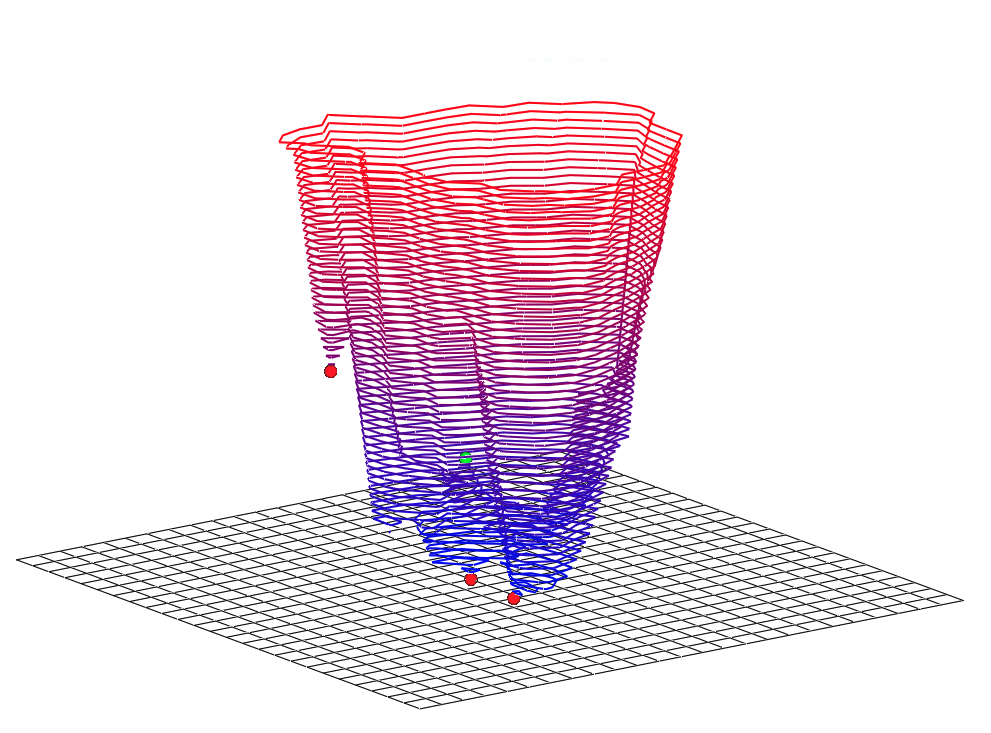
\includegraphics[width=3.5in]{Images/ResNet-Random-3d-contours-critical-points.png}
			\end{array}$
	\end{center}
	\caption{ The 3D loss landscapes with critical points of the ResNet-50 model using random direction iteration for dimensionality reduction. } \label{fig:coparison_of_landscapes}
\end{figure}

\section{Conclusions}
We implemented methods described in "Visualizing the Loss Landscape of Neural Nets" (\url{https://arxiv.org/pdf/1712.09913.pdf}) for creating loss landscapes of artificial neural networks using multiple methods of dimensionality reduction. Next, we visualized our results in OpenGL using a mixture of contour lines and meshes, which we found to create the most easily understood representations of the data. Within the loss landscape, we visualized the path of gradient descent for our models and saw the expected paths, adding a layer of confidence that our loss landscapes were accurate. Finally, we were able to make generalizations about the trainability of the VGG-11 and ResNet-50 models based on the observations from the loss landscapes.

\bibliographystyle{acmsiggraph}
\nocite{*}
\bibliography{final_project_references}

\section{Appendix}
\begin{longtable}{ |p{1.5cm}|p{1.5cm}||p{6.5cm}|p{6.5cm}|  }
 \hline
 \multicolumn{4}{|c|}{\textbf{Table 1: Loss Landscapes}} \\
 \hline
 \textbf{Strategy} & \textbf{Reduction} & \textbf{ResNet-50} & \textbf{VGG-11}\\
 \hline
 2D Contour Lines   
 & Random Direction Iteration
 & \parbox[c]{1em}{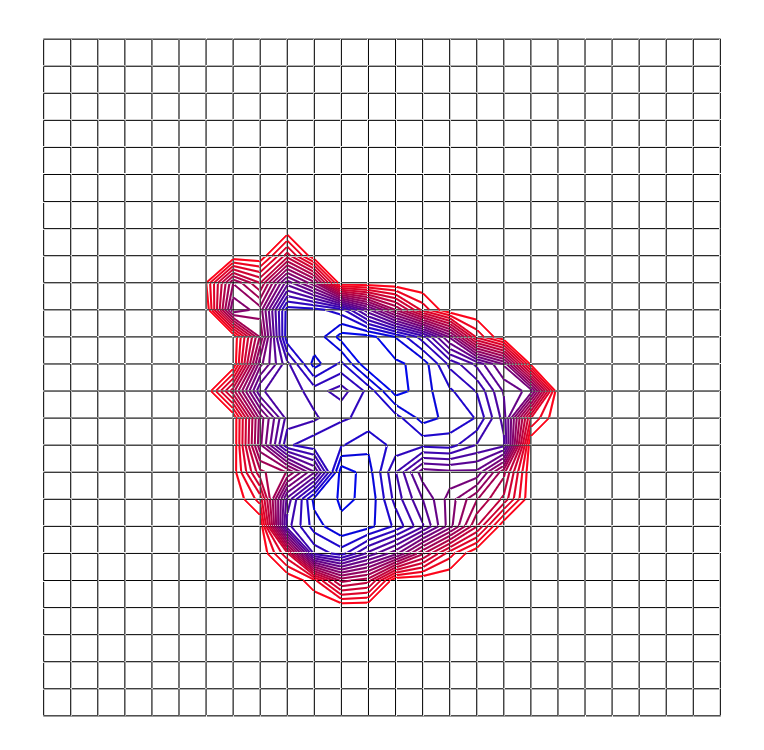
\includegraphics[width=2.6in, trim=0 0 0 -5]{Images/ResNet-Random-2d-contours.png}} 
 & \parbox[c]{1em}{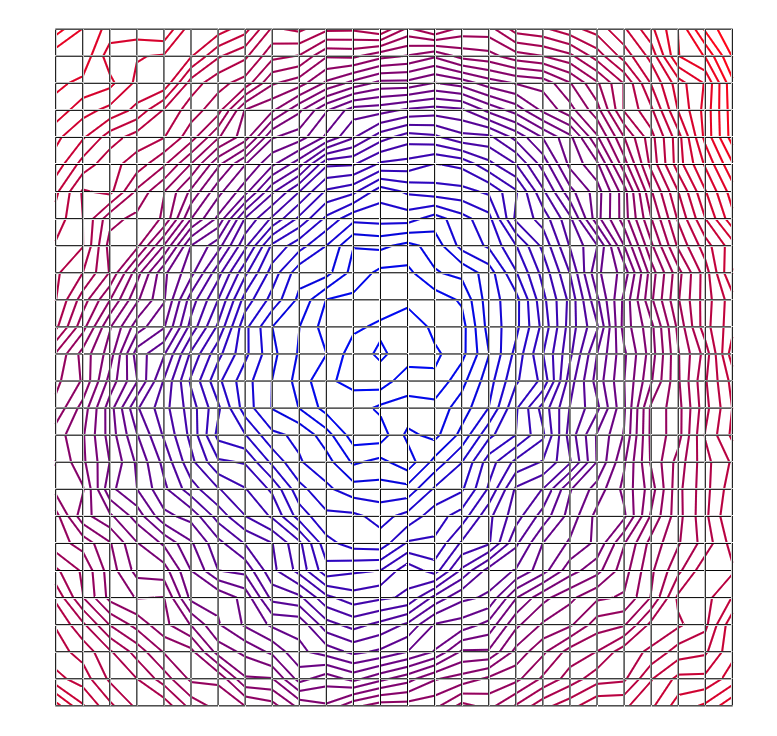
\includegraphics[width=2.6in, trim=0 0 0 -5]{Images/VGG-Random-2d-contours.png}}
 \\
 \hline
 2D Contour Lines   
 & PCA
 & \parbox[c]{1em}{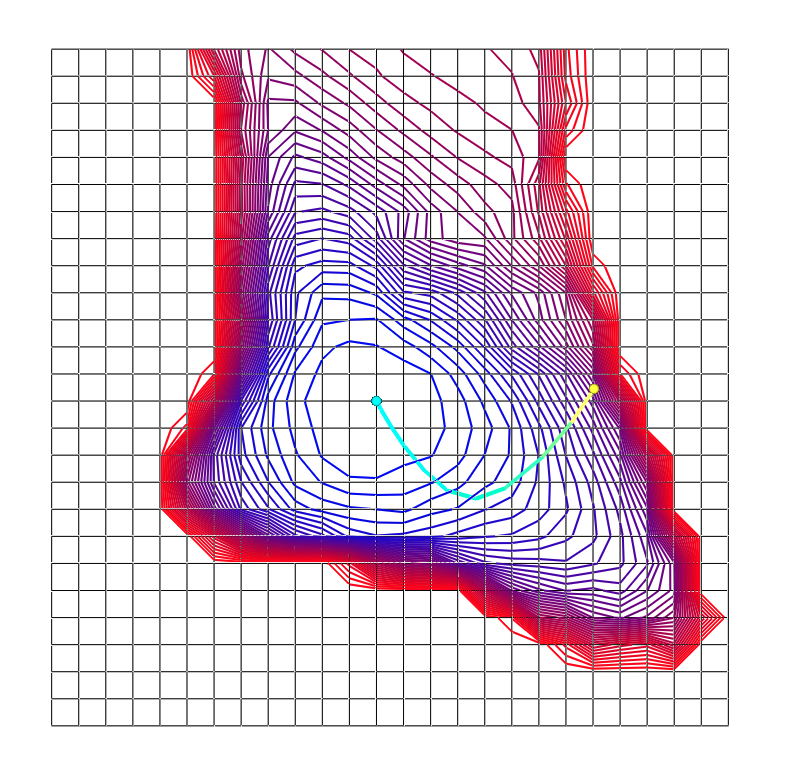
\includegraphics[width=2.6in, trim=0 0 0 -5]{Images/ResNet-PCA-2d-contours.png}} 
 & \parbox[c]{1em}{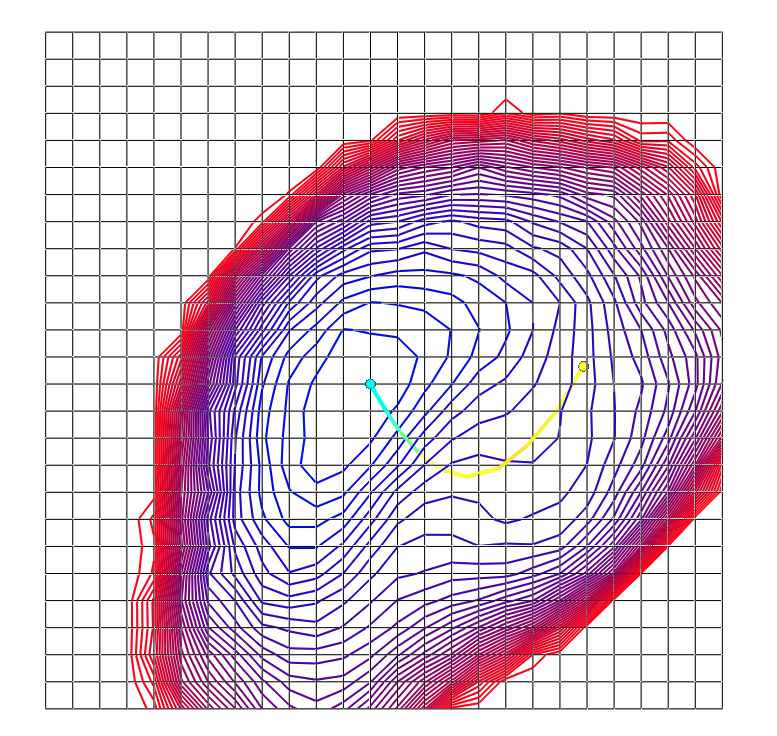
\includegraphics[width=2.6in, trim=0 0 0 -5]{Images/VGG-PCA-2d-contours.png}}
 \\
 \hline
 3D Contour Lines   
 & Random Direction Iteration
 & \parbox[c]{1em}{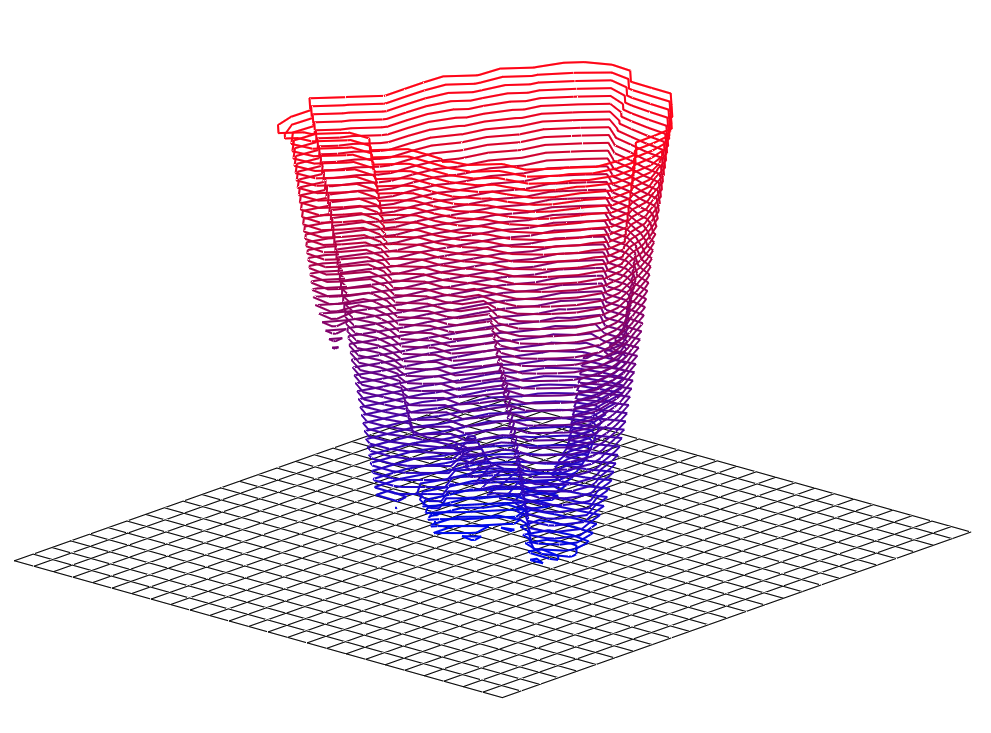
\includegraphics[width=2.6in, trim=0 0 0 -5]{Images/ResNet-Random-3d-contours.png}} 
 & \parbox[c]{1em}{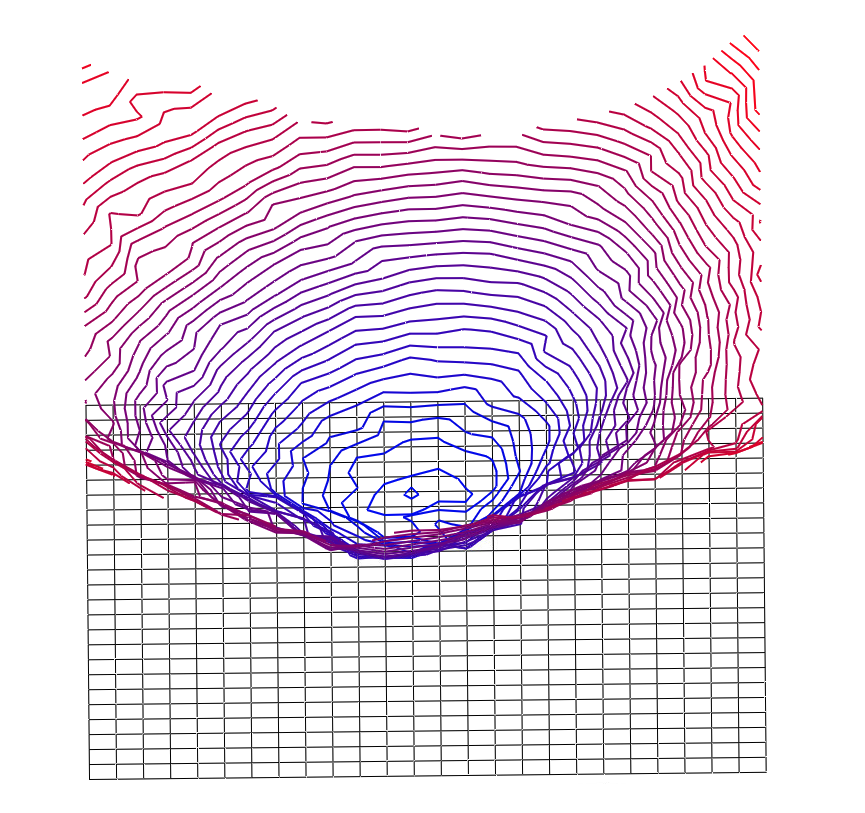
\includegraphics[width=2.6in, trim=0 0 0 -5]{Images/VGG-Random-3d-contours.png}}
 \\
 \hline
 3D Contour Lines   
 & PCA
 & \parbox[c]{1em}{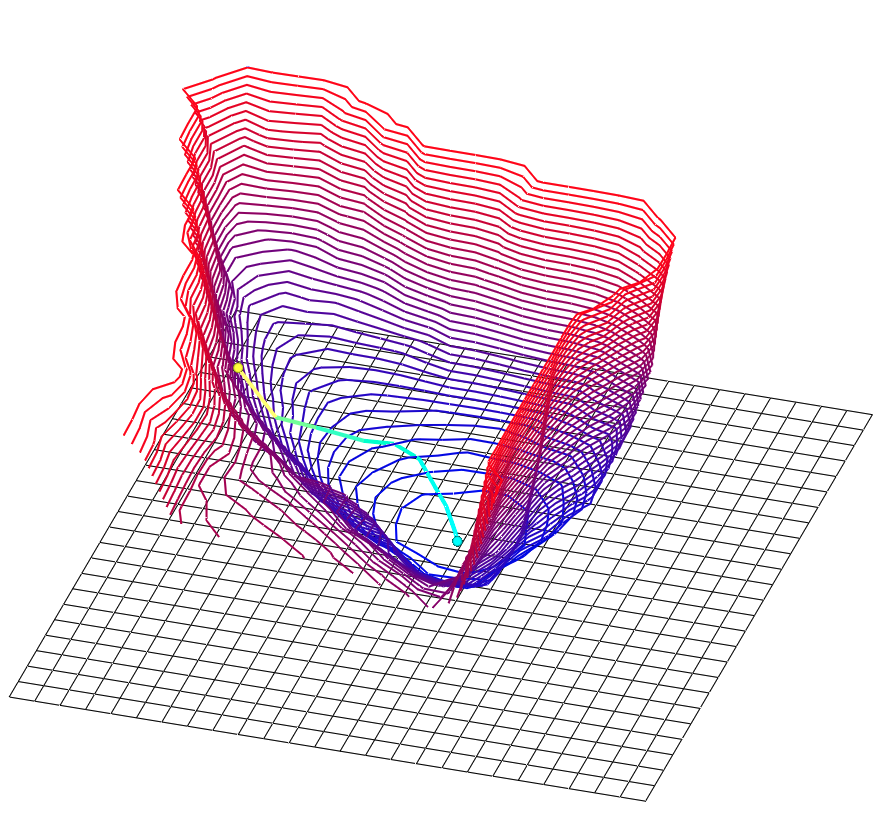
\includegraphics[width=2.6in, trim=0 0 0 -5]{Images/ResNet-PCA-3d-contours.png}} 
 & \parbox[c]{1em}{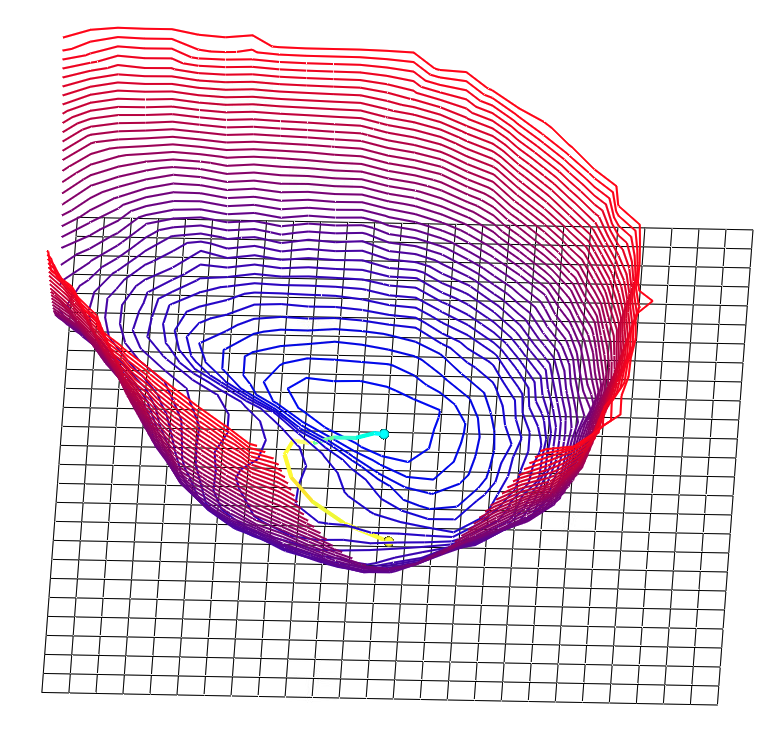
\includegraphics[width=2.6in, trim=0 0 0 -5]{Images/VGG-PCA-3d-contours.png}}
 \\
 \hline
 3D Mesh  
 & Random Direction Iteration
 & \parbox[c]{1em}{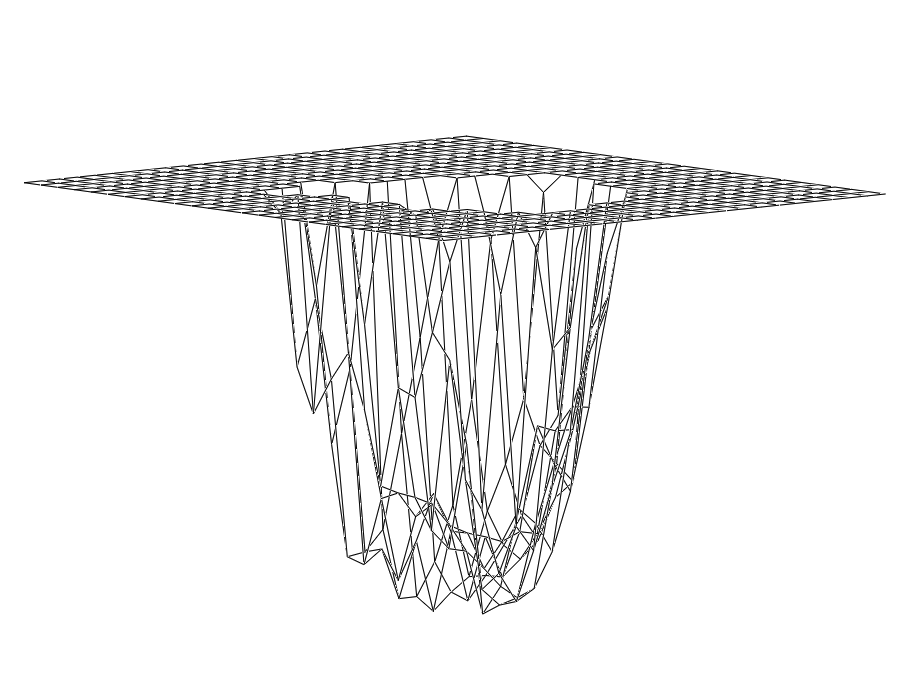
\includegraphics[width=2.6in, trim=0 0 0 -5]{Images/ResNet-Random-3d-mesh.png}} 
 & \parbox[c]{1em}{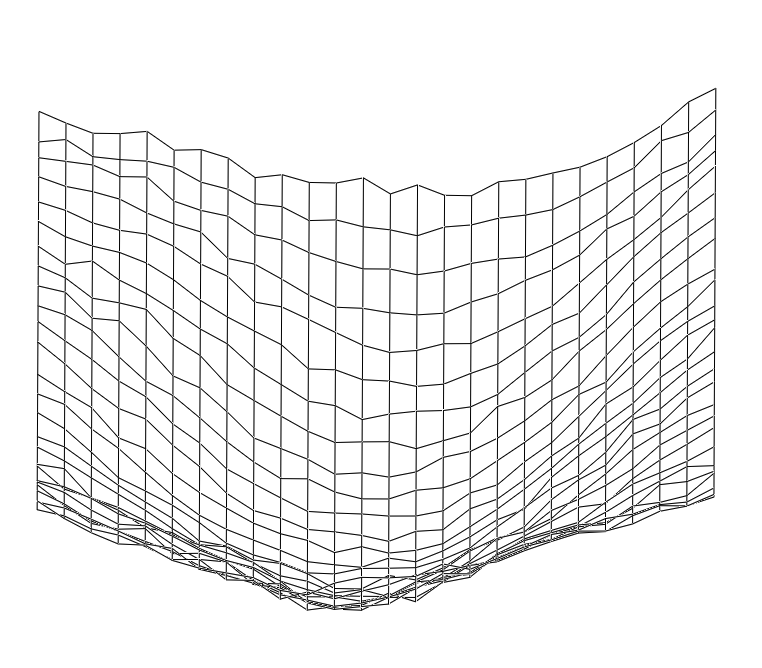
\includegraphics[width=2.6in, trim=0 0 0 -5]{Images/VGG-Random-3d-mesh.png}}
 \\
 \hline
 3D Mesh  
 & PCA
 & \parbox[c]{1em}{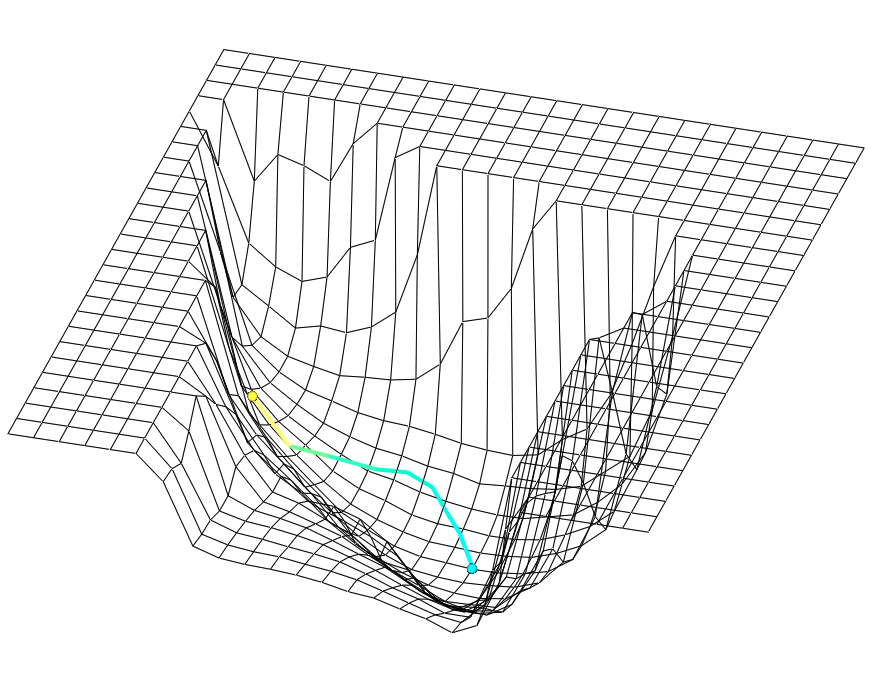
\includegraphics[width=2.6in, trim=0 0 0 -5]{Images/ResNet-PCA-3d-mesh.png}} 
 & \parbox[c]{1em}{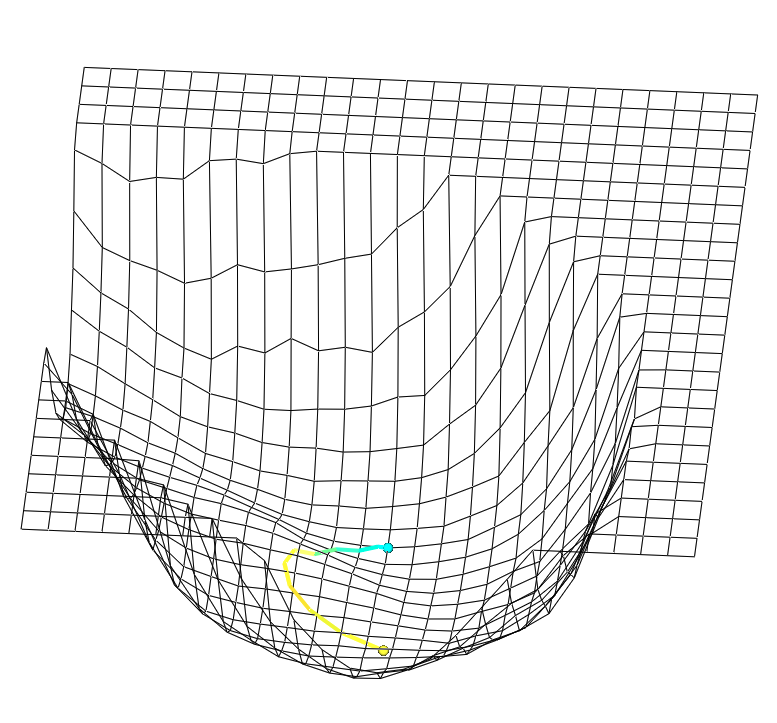
\includegraphics[width=2.6in, trim=0 0 0 -5]{Images/VGG-PCA-3d-mesh.png}}
 \\
 \hline
\end{longtable}

\end{document}


